% !TEX encoding = UTF-8
% !TEX TS-program = pdflatex
% !TEX root = ../tesi.tex
% !TEX spellcheck = it-IT

%**************************************************************
\chapter{Profilo Aziendale}
\label{cap:introduzione}
%**************************************************************

Lo stage formativo si è svolto presso l'azienda \textbf{Nextep S.r.l.}\footnote{\url{http://www.nextep.it/}}, con sede a Carmignano di Brenta(PD). \textbf{Nextep} è una società fondata nel 2000 che opera nel settore dell'informatica e della comunicazione. Il \textit{core business} è riconosciuto nelle attività di progettazione, realizzazione e gestione di infrastrutture di \textit{Information e Digital Communication Technology.}\\
L'azienda è suddivisa in due divisioni principali:
\begin{itemize}
	\item Divisione \textit{marketing} e commerciale: si occupa di studiare il mercato e la clientela;
	\item Divisione tecnica: si occupa della gestione e la realizzazione dei progetti.
\end{itemize}

\begin{figure}[h]
\centering
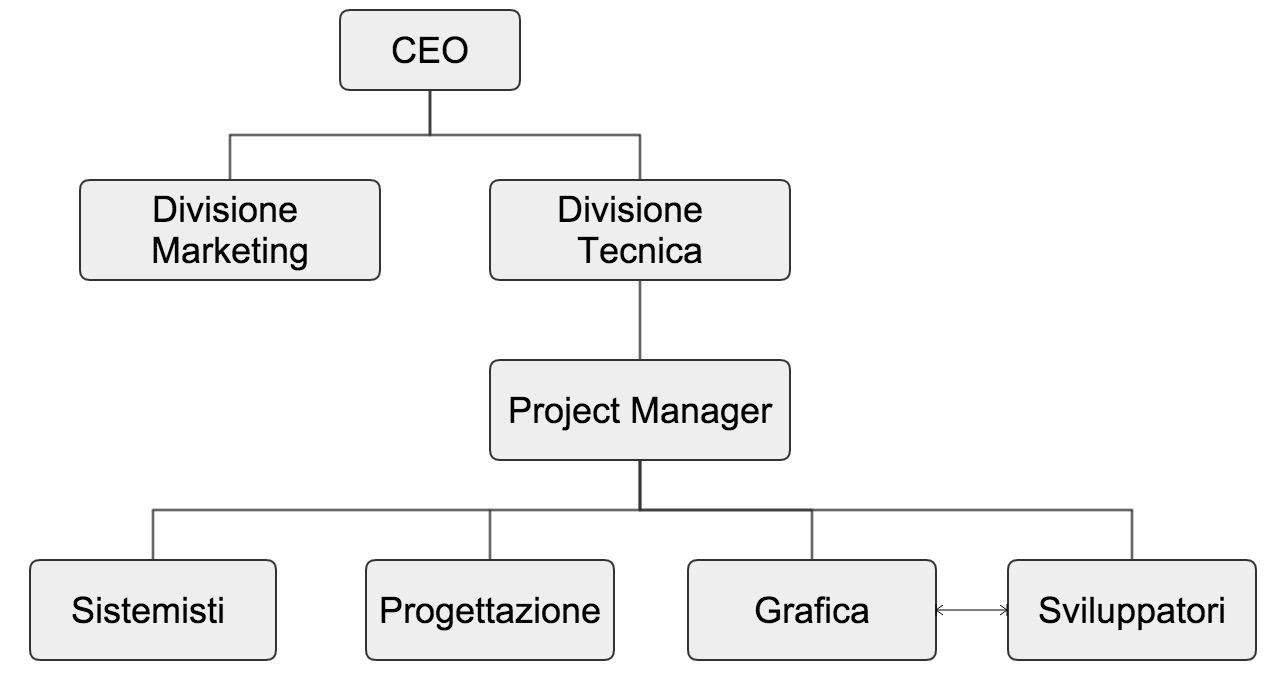
\includegraphics[width=0.8\linewidth]{immagini/organigramma}
\caption[Organigramma dell'azienda]{Organigramma dell'azienda}
\label{fig:logo-nextep}
\end{figure}

L'organico di \textbf{Nextep S.r.l.} è formato da circa 20 persone, suddivisi tra grafici, sviluppatori, marketing e sistemisti. L'azienda fa parte del gruppo Allos\footnote{\url{http://www.allos.it/}} che insieme a Zero12\footnote{\url{http://www.zero12.it/}} condividono l'ambiente di lavoro. Ciò che ne risulta è un ambiente di \textit{coworking} dove si condividono esperienze e conoscenze. Non è raro che le tre aziende collaborano tra di loro per la realizzazione di alcuni progetti.


%**************************************************************
\section{Prodotti e servizi offerti}

L'azienda offre soluzioni innovative che permettono ai cliente di affrontare il mercato con una marcia tecnologica in più sia legata all'innovazione di prodotto che ai processi interni di pianificazione e produzione.

%**************************************************************
\subsection{Prodotti}

Il settore principale di \textbf{Nextep S.r.l. }è il web. Nello specifico l'azienda si occupa di:
\begin{itemize}
	\item Progettazione e sviluppo di siti web e portali;
	\item Progettazione e sviluppo di \textit{Social Intranet }e capitalizzazione della cultura aziendale;
	\item Progettazione e sviluppo di soluzioni \textit{e-commerce};
	\item Progettazione e realizzazione di applicazioni \textit{mobile};
	\item Studio e progettazione della grafica /\textit{user experience};
	\item Integrazione con tecnologie e servizi di \textit{cloud computing};
	\item Analisi, ideazione e realizzazione di azioni di \textit{web markenting}.
\end{itemize}

\begin{figure}[h]
\centering
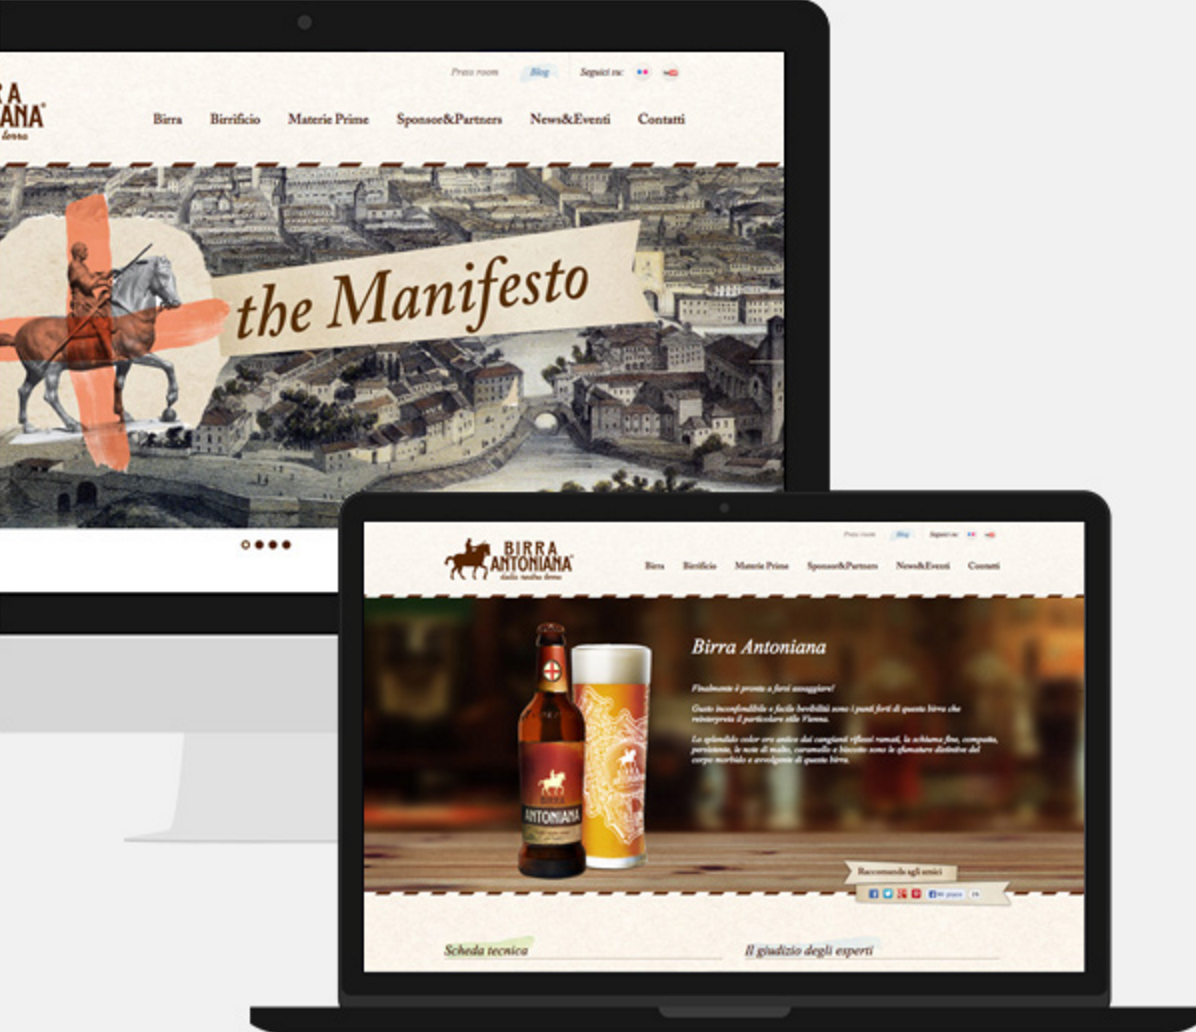
\includegraphics[width=0.5\linewidth]{immagini/sito}
\caption[Birra Antoniana: uno dei siti realizzati da Nextep]{Birra Antoniana: uno dei siti realizzati da Nextep}
\label{fig:sito}
\end{figure}
L'azienda offre un sevizio innovativo di \textit{web design}, marketing e grafica, visibile su tutte le piattaforme e su tutti i dispositivi, quali \textit{smartphone} e \textit{tablet} . Offre diverse soluzioni a seconda delle necessità del cliente; in particolare propone interfacce semplici per la gestione dei contenuti e un design evoluto e personalizzato.


%**************************************************************
\subsection{Servizi}

I principali servizi offerti da \textbf{Nextep S.r.l. }ai propri clienti sono:
\begin{itemize}
	\item Fornitura di servizi a canone (server virtuali, applicazioni web, servizi di \textit{monitoring }di infrastrutture \gls{ict}, \textit{backup-online}, canoni di assistenza e manutenzione dei sistemi, canoni di gestione dei sistemi);
	\item Elaborazione dati, analisi e supporto decisionale in ambito \textit{web marketing, social marketing e social intranet};
	\item Consulenza e formazione di \textit{web marketing, social marketing, web analytics};
	\item Servizio Clienti, attività di supporto tecnico e di gestione di infrastrutture \gls{ict} e siti web.
\end{itemize}

\section{Tecnologia di riferimento}
Le tecnologie maggiormente utilizzate per lo sviluppo dei progetti sono le seguenti:
\begin{itemize}
	\item \textbf{Linguaggi di programmazione: }
	\begin{itemize}
		\item \textbf{Php: }linguaggio più utilizzato per la realizzazione dei \textit{Web-service};
		\item \textbf{Java, Scala: }linguaggi utilizzati per le \textit{Web-application};
		\item \textbf{HTML, CSS, Javascript: }linguaggi utilizzati per la scrittura di pagine web.
	\end{itemize}
	\item \textbf{Framework e CMS: }per facilitare lo sviluppo e il riutilizzo del codice delle proprie applicazioni \textbf{Nextep }utilizza vari \gls{framework} e \gls{cms}:
	\begin{itemize}
		\item \textbf{Play: }web \gls{framework} scritto in Scala. Permette di scrivere applicativi web sia in linguaggio Java che Scala. Segue il \textit{pattern }\gls{mvc};
		\item \textbf{Bootstrap: }si tratta del \gls{framework} \textit{front-end }più utilizzato. Permette di scrivere pagine \textit{web responsive};
		\item \textbf{Compass: }\gls{framework} che fornisce delle estensioni CSS3. Permette di organizzare il CSS in maniera migliore ed aumentare la facilità di manutenzione;
		\item \textbf{Drupal: }si tratta del più popolare \gls{cms} PHP. Permette di avere un riutilizzo sistematico del codice scritto e quindi di ridurre i tempi di sviluppo e manutenzione.
	\end{itemize}
	\item \textbf{Database: }il database viene scelto tenendo conto dei vantaggi/svantaggi di ognuno dei database elencati sotto:
	\begin{itemize}
		\item \textbf{OrientDB: }è un multi-model \textit{No-Sql }\textit{database }scritto in Java;
		\item \textbf{MongoDB: }\textit{database} \textit{NO-SQL}, particolarmente adatto quando vengono gestite grandi quantità di dati;
		\item \textbf{MySQL, SQL Server, PostGreeSQL }: \textit{database }\textit{SQL}.
	\end{itemize}
\end{itemize}
\begin{figure}[h]
\centering
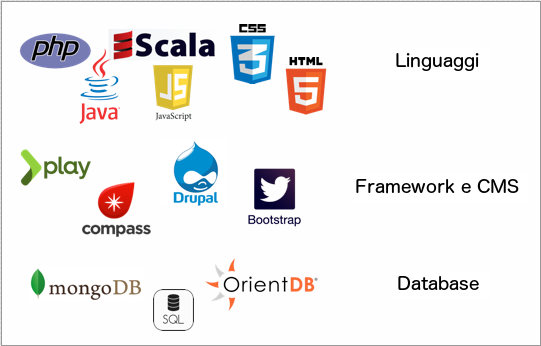
\includegraphics[width=0.6\linewidth]{immagini/White}
\caption[Classificazione delle tecnologie utilizzate]{Classificazione delle tecnologie utilizzate}
\label{fig:White}
\end{figure}


\section{Processi aziendali}
\subsection{Metodologia agile}
L'azienda utilizza una gestione dei progetti seguendo un metodo \textit{agile}\footnote{\url{http://agilemanifesto.org/}}, in quanto per la particolarità del servizio offerto, è più importante mantenere una collaborazione con il cliente rendendolo partecipe nel progetto offrendo cosi una rapida reattività alle nuove richieste. I principi su cui si basa il modello di tipo \textit{agile} sono:
\begin{itemize}
	\item Gli individui  e le iterazione rispetto ai processi  e agli strumenti;
	\item Software funzionante rispetto ad un'ampia documentazione;
	\item Committenti e sviluppatori devono lavorare insieme per tutta la durata del progetto;
	\item La pronta risposta ai cambiamenti rispetto all'esecuzione di un piano.
\end{itemize}

\begin{figure}[h]
\centering
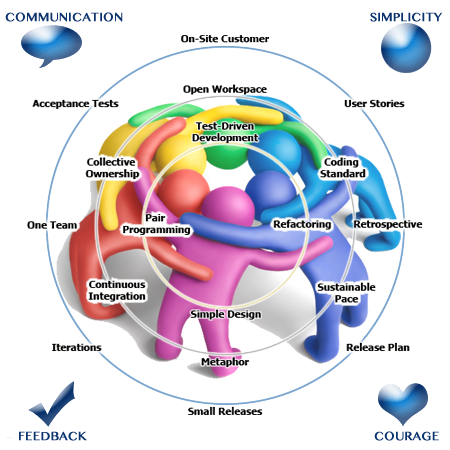
\includegraphics[width=0.7\linewidth]{immagini/agile}
\caption[Raffigurazione della metodologia agile]{Raffigurazione della metodologia agile. Questa immagine è stata presa dall'\href{URL}{articolo sulla metodologia \textit{Agile}}}
\label{fig:agile}
\end{figure}

Nello specifico il team di sviluppo segue un approccio Scrum\footnote{\url{https://it.wikipedia.org/wiki/Scrum_(informatica)}} per i progetti più complessi. Questo modello è basato sui seguenti concetti:
\begin{itemize}
	\item \textbf{Sprint: }rappresenta un'unità base dello sviluppo \textit{Scrum }ed ha una durata fissa. Durante uno \textit{sprint }non è possibile modificare gli obiettivi precedentemente pianificati;
	\item\textbf{Riunioni: }
	\begin{itemize}
		\item Prima dello \textit{sprint }in modo da pianificare gli obiettivi e i tempi stimati per il successivo \textit{sprint};
		\item Dopo lo \textit{sprint }per verificare il lavoro svolto;
		\item Quotidianamente;
		\item Riunioni con i cliente per capire a fondo i requisiti richiesti.
	\end{itemize}
	\item \textbf{Product Backlog: }rappresenta ciò che deve essere fatto in una lista ordinata di requisiti relativi ad un prodotto software, ognuno dei quali avente una priorità;
	\item \textbf{Sprint Backlog: }lista del lavoro che deve essere effettuato nel corso dello \textit{sprint }successivo;
	\item \textbf{Incremento: }è la somma di tutti gli elementi del \textit{Product Backlog }completati duranti gli \textit{sprint} precedenti;
	\item \textbf{Burn down: }è la rappresentazione grafica del lavoro da fare per il progetto visto rispetto al tempo.
\end{itemize}

\begin{figure}[h]
\centering
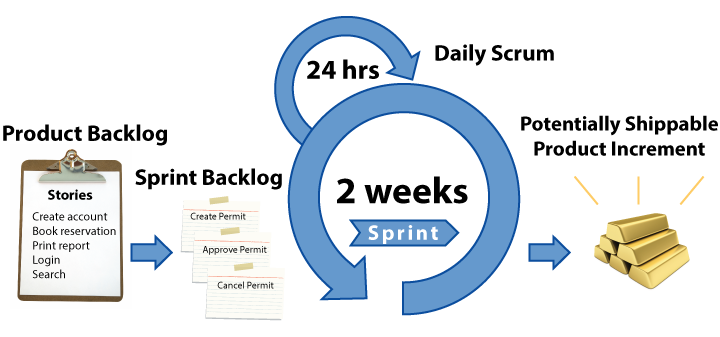
\includegraphics[width=0.8\linewidth]{immagini/scrum}
\caption[Una panoramica su scrum]{Una panoramica su scrum. Questa immagine è stata presa dall'\href{http://www.agilenutshell.com/scrum}{articolo "\textit{Agile In a Nutshell}"}}
\label{fig:scrum}
\end{figure}


Non essendo un gruppo molto ampio, questo modello si adatta molto bene all'azienda e questo permette di reagire velocemente ai cambiamenti dei requisiti che si verificano durante lo sviluppo software diventando più flessibile.

\subsection{Strumenti a supporto dei processi}
\subsection*{Gestione di progetto}
Nextep utilizza \textit{Zendesk}\footnote{\url{https://www.zendesk.it/}} per fornire assistenza ai clienti attraverso diversi canali, tra cui \textit{email, telefono, chat, web e social media}. Tutte le iterazioni su Zendesk sono tracciate fornendo dati importanti dell'azienda cosi come un'analisi della performance individuale. In questo modo si ha una visione ampia su come sta andando il lavoro svolto.

\begin{figure}[h]
\centering
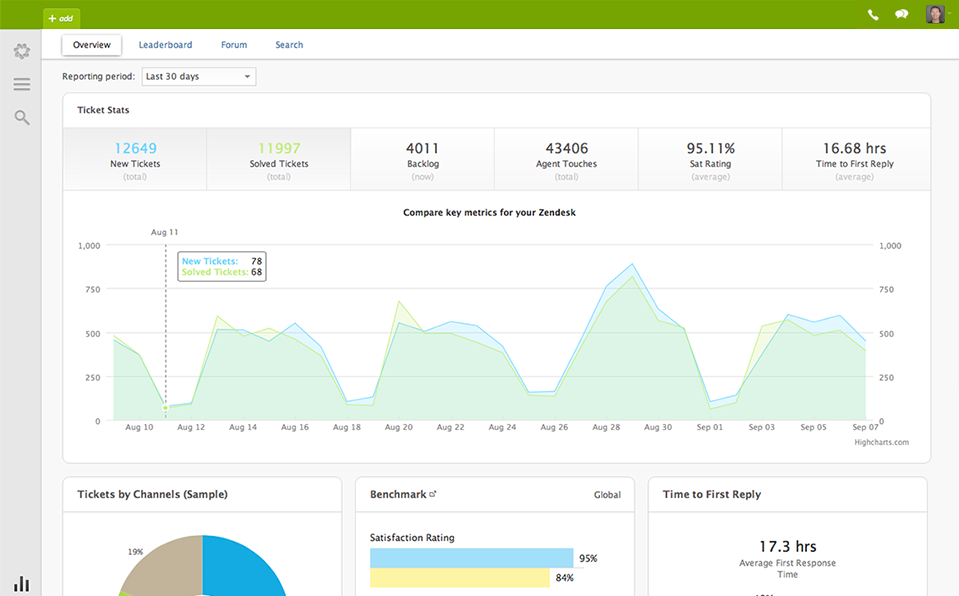
\includegraphics[width=0.8\linewidth]{immagini/reporting}
\caption[Esempio Report Zendesk]{Esempio Report Zendesk}
\label{fig:reporting}
\end{figure}

\newpage
Per la gestione di progetto viene utilizzato Jira Agile\footnote{\url{https://jira.atlassian.com/secure/Dashboard.jspa}} seguendo il modello delle \textit{user story}. Jira è un tool per la pianificazione, organizzazione e verifica del lavoro. Esso permette di:
\begin{itemize}
	\item Gestire e assegnare \textit{ticket};
	\item Integrare i progetti con il sistema di versionamento \gls{git}\footnote{\url{http://git-scm.com/}};
	\item Pianificare le attività;
	\item Gestione dei \textit{task }e delle ore di lavoro.
\end{itemize}

\subsection*{Scrum board}
Una \textit{scrum board }è una lavagna fisica o virtuale per la gestione delle varie attività del processo produttivo. Suddivide in colonne i vari stati evolutivi del prodotto. Ogni colonna può contenere diversi post-it che rappresentano un determinato task. Uno spostamento rappresenta un'evoluzione o una regressione. Questo strumento viene utilizzato dal team di sviluppo per la gestione della produzione e per avere un panorama dello stato di avanzamento dei lavori. I post-it vengono inseriti dai project manager e ogni colore ha una priorità diversa, conosciuto al intero team. \\
La suddivisione degli stati della \textit{Scrum board }è la seguente:

\begin{figure}[h]
\centering
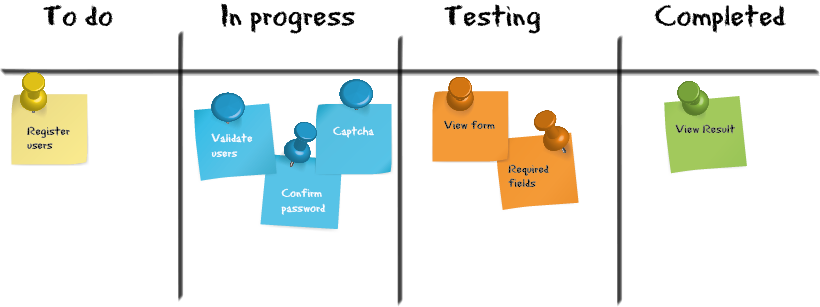
\includegraphics[width=0.9\linewidth]{immagini/scrum-board}
\caption[Scrum board]{Scrum board}
\label{fig:scrum-board}
\end{figure}

\begin{itemize}
	\item \textbf{To Do: }detto anche \textit{backlog }rappresenta un prodotto appena commissionato che deve essere ancora assegnato;
	\item \textbf{In progress: }indica che l'attività è stata presa in carico ed è in fase di sviluppo;
	\item \textbf{Testing: }indica la terminazione dello sviluppo e l'inizio della fase di \textit{testing};
	\item \textbf{Completed: }il prodotto finito è stato approvato.
\end{itemize}

\subsection*{Documentazione}
Per la realizzazione dei documenti inerenti ai progetti viene utilizzato Google Docs. In questo modo permette a più dipendenti di collaborare allo stesso documento, anche contemporaneamente,ed è accessibile a tutti attraverso il browser. È possibile utilizzare la cronologia delle revisioni per vedere le vecchie versioni e in base alla persona che ha effettuato la modifica.

\subsection*{Sistema di versionamento}
Come sistema di versionamento Nextep utilizza \gls{git}.\\
I \textit{repository }dei progetti si trovano su dei server gestiti dai dipendenti dell'azienda.

\subsection*{Ambiente di sviluppo}
L'ambiente di sviluppo varia a seconda delle tecnologie coinvolte nel progetto proposto.\\
Vengono utilizzati i seguenti \gls{IDE}:
\begin{itemize}
	\item \textbf{Eclipse/IntelliJ: }per lo sviluppo di applicazioni in Java/Scala;
	\item \textbf{Smultron/PhpStorm: }per lo sviluppo di applicazioni in Php;
	\item \textbf{Sublime Text: }per lo sviluppo di codice HTML/CSS/Javascript e Php.
\end{itemize}

\subsection*{Sistemi operativi}
\textbf{Nextep} non impone nessun obbligo sul sistema operativo utilizzato. All'interno dell'azienda i dipendenti utilizzano vari sistemi operativi come \textit{Windows, Linux e Mac OS} a seconda delle proprie preferenze.\\
Nell'ultima settimana di permanenza nell'azienda sono venuto a conoscenza dell'acquisto di vari computer \textit{Mac Book e iMac }per permettere a chi desidera di passare o di fare l'\textit{upgrade }al nuovo \textit{OS X}. Questo non toglie che uno può utilizzare il sistema operativo preferito.\\
I \textit{server }utilizzati per il \textit{deployment }sono solitamente macchine con sistema operativo \textit{Linux Ubuntu} o \textit{Linux Debian} residenti in \textit{Amazon Web Services (AWS).}

\begin{figure}[h]
\centering

\includegraphics[width=0.7\linewidth]{immagini/gestione}
\caption[Classificazione degli strumenti utilizzati]{Classificazione degli strumenti utilizzati}
\label{fig:gestione}
\end{figure}

\newpage
\section{Tipologia di clientela e propensione all'innovazione}
L'azienda offre i propri servizi a diverse tipologie di clientela: dalle piccole aziende e i singoli professionisti, alle medie e grandi aziende. I principali clienti sono aziende italiane del settore \textit{retail}, manifatturiero e \textit{corporate}. \\
Per l'azienda è importante innovare per restare competitiva e acquisire e/o mantenere una posizione importante sul mercato, specialmente lavorando nell'ambito del Web. In tal senso, \textbf{Nextep }sta cercando persone che abbiano un'attitudine positiva verso il cambiamento, spingendo loro a proporre soluzioni innovative. Anche lo spazio di \textit{coworking} in cui ha sede \textbf{Nextep} è luogo di condivisione. Infatti, le aziende si confrontano su possibili progetti oppure nuove opportunità su cui lavorare assieme, trasformando lo spazio collaborativo in un proprio laboratorio di innovazione. Oltre alle riunioni e ai vantaggi offerti dall'ambiente di lavoro condiviso, l'azienda svolge dei corsi di formazione del personale con lo scopo di mantenere coinvolto e motivato l'intero \textit{team}.